\documentclass[11pt,a4paper]{article}
\usepackage[margin=2.3cm]{geometry}
\usepackage{amsmath,amssymb,amsthm,mathtools,bm}
\usepackage{booktabs,array,tabularx}
\usepackage{enumitem}
\usepackage{algorithm}
\usepackage[noend]{algpseudocode}
\usepackage[dvipsnames]{xcolor}
\usepackage{pgfplots}
\pgfplotsset{compat=1.17}
\usepackage[colorlinks=true,linkcolor=NavyBlue,citecolor=NavyBlue,urlcolor=NavyBlue]{hyperref}
\usepackage{tcolorbox}
\usepackage{float}

\newtheorem{proposition}{Proposition}
\newtheorem{lemma}{Lemma}
\newtheorem{assumption}{Assumption}
\theoremstyle{definition}
\newtheorem{definition}{Definition}
\newtheorem{requirement}{Requirement}
\renewcommand{\therequirement}{R\arabic{requirement}}
\theoremstyle{remark}
\newtheorem{remark}{Remark}

\newtcolorbox{principle}{colback=gray!6,colframe=gray!50,boxrule=0.4pt,arc=1pt,left=6pt,right=6pt,top=4pt,bottom=4pt}
\newtcolorbox{decision}{colback=NavyBlue!4,colframe=NavyBlue!50,boxrule=0.4pt,arc=1pt,left=6pt,right=6pt,top=4pt,bottom=4pt}

\newcommand{\R}{\mathbb{R}}
\newcommand{\E}{\mathbb{E}}
\newcommand{\Prob}{\mathbb{P}}
\newcommand{\T}{^{\top}}
\newcommand{\one}{\mathbf{1}}
\newcommand{\zm}{z_{\mathrm{med}}}
\newcommand{\Wo}{W_0}
\newcommand{\bx}{\bm{x}}
\newcommand{\bh}{\bm{h}}
\newcommand{\bff}{\bm{f}}
\newcommand{\Pm}{\bm{P}}
\newcommand{\Qm}{\bm{Q}}
\newcommand{\btheta}{\bm{\Theta}}
\newcommand{\Win}{\mathsf{W}}
\newcommand{\Wc}{\mathsf{W}^{\mathrm{cv}}}
\newcommand{\Dl}{\mathsf{D}^{\ell}}
\newcommand{\Dn}{\mathsf{D}}
\newcommand{\Dcv}{\mathsf{D}^{\mathrm{2nd}}}
\newcommand{\NT}{\mathsf{N}}
\newcommand{\lmexp}{\operatorname{log1mexp}}

\title{A Censored Cover Model for RFQ Pricing\\[3pt]
\large Fair charge, win probability, daily calibration and intraday filtering\\[2pt]
\normalsize Technical specification --- draft v0.4}
\author{}
\date{26 October 2026}

\begin{document}
\maketitle

\begin{abstract}
We specify a model for dealer-to-client bond RFQs that delivers, for every inquiry, (i) a \emph{fair charge}, defined as the median of the best competing charge over a reference mid, and (ii) a full win-probability curve $s\mapsto\Prob(\text{win}\mid s)$. The latent object is the \emph{cover} $C$, the best competing charge. Wins, wins with a disclosed cover, losses matched to the public tape and losses without a level are all treated as partial (censored) observations of this one quantity. The cover follows a smallest-extreme-value (Gumbel-min) law. Section~\ref{sec:distribution} motivates this choice from the structure of the data (the cover is a minimum of competing quotes, and most observations are censored), derives its properties and maps each record type onto it. The fair charge is multiplicative: a per-bond fair charge at a reference size, made of a per-country maturity curve with a curvature penalty between consecutive maturities times an idiosyncratic bond spread, times a size curve and multipliers for tier, client, venue, side and trading session. Liquidity, age and similar bond characteristics are not modelled explicitly; they are absorbed by the idiosyncratic spread. Each morning the model is fitted by penalised maximum likelihood with partial pooling; during the day a subset of log-effects is treated as a random-walk state and updated after each resolved inquiry with a rank-one Laplace filter.
\end{abstract}

\begin{principle}
\textbf{Design principles.}
\begin{enumerate}[leftmargin=*,itemsep=1pt]
\item Model the level to beat, not the win flag. Every outcome type is an observation of the same latent cover, with the appropriate censoring.
\item Interpretability is a constraint: outputs are a per-bond fair charge and multiplicative adjustments that a trader can read and override.
\item Partial pooling everywhere: sparse bonds and clients shrink toward their country curve and tier; data-rich ones are free to deviate.
\item No engineered bond characteristics: the bond's own history, through its idiosyncratic spread, carries liquidity, age and benchmark status.
\item One model, two clocks: a morning batch fit and an intraday filter on the same likelihood.
\end{enumerate}
\end{principle}

\tableofcontents

%======================================================================
\section{Setup and notation}
%======================================================================

\subsection{Inquiry record}
An inquiry $i$ is a request for quote received at time $t_i$. It carries:
\begin{center}
\begin{tabularx}{\textwidth}{>{$}l<{$}X}
\toprule
b(i) & bond, with country $g(b)$ and time to maturity $T_b$ (years, recomputed daily) \\
c(i),\,k(i) & client and client tier, $k(i)=k(c(i))$ \\
v(i) & venue \\
p(i) & trading session: pre (before 08:15), core, post (from 16:30); Section~\ref{sec:session} \\
d_i\in\{+1,-1\} & side: $+1$ if the client buys (we offer), $-1$ if the client sells (we bid) \\
q_i & nominal size; $q^\star_b$ is the reference size for bond $b$ (desk convention, e.g.\ per country) \\
n_i & number of dealers in competition, when disclosed \\
m_i & reference mid (price) at $t_i$; $\mathrm{DV01}_i$ the price value of one basis point \\
P_i & our quoted price \\
O_i & outcome (Table~\ref{tab:outcomes}) and, when available, a level $c_i$ \\
\bottomrule
\end{tabularx}
\end{center}

\subsection{Charges}
All prices are mapped to \emph{charges} relative to the mid, in basis points of yield, positive when the client pays:
\begin{equation}\label{eq:charge}
s_i \;=\; \frac{d_i\,(P_i - m_i)}{\mathrm{DV01}_i}.
\end{equation}
For a desk quoting in price the same definitions hold with $\mathrm{DV01}_i\equiv 1$. Any competing quote, the client's limit and any tape print are mapped with the same convention. A tape print at price $p$ for inquiry $i$ gives the level
\begin{equation}\label{eq:tape}
c_i \;=\; \frac{d_i\,(p - m_{\tau_i})}{\mathrm{DV01}_i},
\end{equation}
where $\tau_i$ is the execution time if the mid history is available (preferred), otherwise $t_i$.

\subsection{Latent levels}
\begin{definition}[Cover, reservation, level to beat]
For inquiry $i$:
\begin{itemize}[itemsep=1pt]
\item $C_i$ is the \emph{cover}: the best (lowest) charge quoted by any competitor;
\item $R_i$ is the client's \emph{reservation charge}: the client trades only if the best quote is at or below $R_i$; $R_i=-\infty$ encodes pure price discovery;
\item $Y_i=\min(C_i,R_i)$ is the \emph{level to beat}.
\end{itemize}
We win if and only if $s_i < Y_i$. The client trades away if $C_i<\min(s_i,R_i)$, and does not trade if $R_i<\min(s_i,C_i)$.
\end{definition}

\subsection{Outcome types}
\begin{table}[H]
\centering
\begin{tabular}{llll}
\toprule
Code & Event & Information on $(C_i,R_i)$ & Type \\
\midrule
$\Win$ & won, no cover disclosed & $C_i>s_i,\;R_i>s_i$ & right-censored \\
$\Wc$ & won, cover $c_i$ disclosed & $C_i=c_i>s_i,\;R_i>s_i$ & exact in $C$ \\
$\Dl$ & done away, level $c_i$ (tape or venue) & $C_i=c_i<s_i,\;R_i\ge c_i$ & exact / interval \\
$\Dn$ & done away, no level & $C_i<s_i,\;R_i\ge C_i$ & left-censored \\
$\Dcv$ & done away, we were second (``covered'') & $C_i<s_i<C^{(2)}_i$ & order statistic \\
$\NT$ & not traded & $R_i<\min(s_i,C_i)$ & reservation \\
\bottomrule
\end{tabular}
\caption{Outcome types. Inquiries where we did not quote are excluded (they carry no $s_i$), but can be added as $\Dl$/$\Dn$ observations with $s_i=+\infty$.}
\label{tab:outcomes}
\end{table}

\subsection{Statistical vocabulary}\label{sec:vocab}
The document uses the vocabulary of survival analysis and of English-language statistics. The terms below are used throughout; French equivalents are given in parentheses.

\begin{description}[itemsep=3pt,leftmargin=0pt]
\item[Location and scale] (\emph{paramètre de position}, \emph{paramètre d'échelle}). A family of distributions is a \emph{location--scale family} if all its members are obtained from one standard random variable $\varepsilon$ by an affine map, $X=\mu+\sigma\varepsilon$ with $\sigma>0$. The \emph{location} $\mu$ slides the distribution along the axis without changing its shape; the \emph{scale} $\sigma$ stretches or compresses it. For the normal law $\mathcal N(\mu,\sigma^2)$ the location is the mean and the scale the standard deviation, but the location can be any fixed point of the distribution (mean, median, mode) depending on how $\varepsilon$ is centred. In this document the cover is written $C_i=F_i+\sigma_i(\varepsilon_i-\zm)$ (Section~\ref{sec:definition}), and
\begin{itemize}[itemsep=1pt]
\item the \textbf{location} is $F_i$, the fair charge, centred so that it is the \emph{median} of the cover: quoting $F_i$ wins half the time given trade;
\item the \textbf{scale} is $\sigma_i$, in bp: the width of the win curve, i.e.\ how many bp it takes for the win probability to go from high to low (one $\sigma_i$ wider than fair wins 15\%, one $\sigma_i$ tighter wins 77\%).
\end{itemize}
``Modelling the location'' therefore means modelling how the fair charge depends on bond, size, client, venue and so on (Section~\ref{sec:location}); ``modelling the scale'' means modelling how steep the win curve is. A \emph{location family} is the special case where the scale is held fixed and only the location varies.
\item[Survival function] (\emph{fonction de survie}). $S(y)=\Prob(C>y)$, one minus the distribution function (\emph{fonction de répartition}). Here $S(s)$ is the probability of winning at charge $s$, given that the client trades.
\item[Hazard and cumulative hazard] (\emph{taux de hasard}, \emph{hasard cumulé}). $\lambda(y)=f(y)/S(y)$ and $\Lambda(y)=-\ln S(y)$. Here: the rate at which the chance of winning is lost per additional bp of charge, and its integral.
\item[Censoring] (\emph{censure}). An observation is \emph{right-censored} when we only know that $C>s$ (a win), \emph{left-censored} when we only know that $C<s$ (a loss without a level), and \emph{interval-censored} when we know that $L<C\le U$ for two known charges (Section~\ref{sec:datamap}).
\item[Likelihood] (\emph{vraisemblance}). The probability the model assigns to what was observed; $\ell_i$ denotes its logarithm for inquiry $i$, and the model is fitted by maximising the sum of the $\ell_i$ plus penalties.
\item[Partial pooling, shrinkage] (\emph{rétrécissement}). Effects of sparse groups (a client with few inquiries, a bond rarely asked) are pulled toward their group value by a Gaussian prior, i.e.\ a quadratic (ridge) penalty; groups with a lot of data are pulled little.
\end{description}

%======================================================================
\section{Assumptions}
%======================================================================

\begin{assumption}[Non-informative censoring]\label{ass:censoring}
Conditionally on the features $\bx_i$ used in the model, our charge $s_i$ is independent of $(C_i,R_i)$.
\end{assumption}
This is the standard survival-analysis condition and the main threat to validity: if traders quote tight precisely when they know the street is tight for reasons not in $\bx_i$, the spread sensitivity is biased. Section~\ref{sec:practical} lists mitigations.

\begin{assumption}[Conditional independence]\label{ass:indep}
$C_i \perp R_i \mid \bx_i$.
\end{assumption}

\begin{assumption}[Exchangeable competitors, optional]\label{ass:iid}
When $n_i$ is known, the $n_i-1$ competing charges $Q_{i1},\dots,Q_{i,n_i-1}$ are i.i.d.\ given $\bx_i$, and $C_i=\min_j Q_{ij}$.
\end{assumption}

%======================================================================
\section{The distribution of the cover}\label{sec:distribution}
%======================================================================

This section is the core of the specification. We first list what our data require of the distribution of $C_i$ (\S\ref{sec:requirements}), then give four independent reasons that point to the smallest-extreme-value law (\S\ref{sec:motivation}), define it (\S\ref{sec:definition}), derive the properties used in the rest of the document (\S\ref{sec:properties}), show how each of our records maps onto it (\S\ref{sec:datamap}), and close with its weaknesses, safeguards and alternatives (\S\ref{sec:limitations}--\S\ref{sec:alternatives}).

%----------------------------------------------------------------------
\subsection{What the data require}\label{sec:requirements}
%----------------------------------------------------------------------
After the mapping \eqref{eq:charge}--\eqref{eq:tape}, each inquiry gives our charge $s_i$, an outcome flag and, for a subset, a noisy level $c_i$. Five features of these data constrain the choice.

\begin{requirement}[Real support]\label{req:support}
Covers through the mid occur (an axed dealer, a stale mid), so $C_i$ must be supported on the whole real line, even if its median is positive.
\end{requirement}

\begin{requirement}[A minimum of competing quotes]\label{req:min}
$C_i$ is the best of several dealers' quotes, possibly capped by the client's limit. Its distribution should have the shape of a minimum (skewed toward tight levels: one dealer can be very tight, but the best of several is rarely very wide) and should behave consistently when the number of dealers or the presence of a client limit changes.
\end{requirement}

\begin{requirement}[Censoring dominates]\label{req:censoring}
Most records are bounds, not levels: a win only says $C_i>s_i$, a loss without a matched print only says $C_i<s_i$. The survival function $S(y)=\Prob(C_i>y)$, its logarithm and differences $S(a)-S(b)$ must be available in closed form and be numerically stable, because they are evaluated millions of times in the daily fit and once per event in the intraday filter.
\end{requirement}

\begin{requirement}[Well-posed estimation and decision]\label{req:concave}
Each record's log-likelihood should be concave in the location, so that one-dimensional updates (the intraday filter) have a unique solution, and the expected-P\&L problem should have a unique optimum, ideally in closed form.
\end{requirement}

\begin{requirement}[Interpretable parameters]\label{req:interp}
A location equal to the fair charge (median, so that ``fair'' means a 50\% hit ratio given trade), a scale equal to the width of the win curve, and covariate effects that act multiplicatively on the fair charge.
\end{requirement}

%----------------------------------------------------------------------
\subsection{Motivation: four routes to the same law}\label{sec:motivation}
%----------------------------------------------------------------------

\paragraph{(a) Extreme-value theory.} The cover is a minimum, $C_i=\min_{j\le N}Q_{ij}$. Whatever the distribution of an individual dealer's quote, provided its lower tail is lighter than a power law (normal, logistic, exponential-type tails all qualify), the Fisher--Tippett--Gnedenko theorem for minima states that $(C_i-b_N)/a_N$ converges to the standard smallest-extreme-value law as $N$ grows. The shape of the cover is therefore not a modelling whim: it is the generic shape of the best of several quotes. In RFQ protocols $N$ is small (typically 2 to 6), so this asymptotic result motivates the shape rather than justifying it; route (b) makes the law exact.

\paragraph{(b) Exact closure under minima.} If each dealer's quote is itself Gumbel-min with common scale $\sigma$, then the minimum of any number of them is again Gumbel-min with the same scale and a shifted location (Proposition~\ref{prop:minstable}). Among the min-stable laws (the three extreme-value types), Gumbel-min is the only one supported on the whole real line (Requirement~\ref{req:support}). This gives a model that is internally consistent across dealer counts and with a client limit (Requirement~\ref{req:min}): the per-dealer quote, the street cover and the level to beat all live in the same family.

\paragraph{(c) Random utility.} Treat the client as choosing the lowest perceived charge among the quotes. When the perceived charges carry independent Gumbel-min noise, the probability that a given dealer is chosen is a softmax of the medians, and the identity of the winner is independent of the winning level (Proposition~\ref{prop:minstable}). This is McFadden's conditional-logit model, the standard model of discrete choice. It is what makes the reservation model and the factorisation of the ``done away'' likelihood exact (Proposition~\ref{prop:outcomes}), and it explains the logistic win curve as a special case (Proposition~\ref{prop:logistic}).

\paragraph{(d) Survival analysis.} Read the charge as ``time'' and losing the ticket as the ``event''. The Gumbel-min law is the unique location family whose cumulative hazards are proportional across covariates (Proposition~\ref{prop:ph}). Covariate effects on the fair charge are then simultaneously shifts of the win curve and proportional changes of the hazard of losing, so the survival-analysis toolkit (censored likelihoods, Kaplan--Meier and Turnbull estimators, log-cumulative-hazard plots) applies without modification.

%----------------------------------------------------------------------
\subsection{Definition and parameterisation}\label{sec:definition}
%----------------------------------------------------------------------
Let $\varepsilon$ follow the standard smallest-extreme-value law, $\Prob(\varepsilon>z)=\exp(-e^{z})$, whose median is
\[
\zm=\ln\ln 2\approx -0.3665 .
\]
We parameterise the cover by its median $F_i$ and a scale $\sigma_i>0$:
\begin{equation}\label{eq:cover}
C_i \;=\; F_i + \sigma_i\,(\varepsilon_i - \zm),\qquad \varepsilon_i\sim\mathrm{SEV}(0,1).
\end{equation}
$F_i=\operatorname{median}(C_i\mid\bx_i)$ is the \textbf{fair charge}. Define the standardised level
\begin{equation}\label{eq:z}
z_i(y) \;=\; \frac{y-F_i}{\sigma_i}+\zm .
\end{equation}
Then
\begin{align}
S_{C}(y) &= \Prob(C_i>y) = \exp\!\bigl(-e^{z_i(y)}\bigr), \label{eq:S}\\
f_{C}(y) &= \sigma_i^{-1}\,e^{z_i(y)}\exp\!\bigl(-e^{z_i(y)}\bigr), \label{eq:f}\\
\Lambda_C(y) &= -\ln S_C(y)=e^{z_i(y)}=\ln 2\cdot e^{(y-F_i)/\sigma_i}, \label{eq:cumhaz}\\
\lambda_C(y) &= f_C(y)/S_C(y)=\sigma_i^{-1}e^{z_i(y)}, \label{eq:hazard}\\
y_i(p) &= F_i+\sigma_i\bigl(\ln(-\ln p)-\zm\bigr)\quad\text{solves } S_C(y)=p. \label{eq:quantile}
\end{align}
Measuring the charge in units of $\sigma_i$ away from fair, $s=F_i+k\sigma_i$, the win probability given trade takes a form that can be read on a desk:
\begin{equation}\label{eq:twopower}
\boxed{\;\Prob\bigl(C_i>F_i+k\sigma_i\bigr)\;=\;2^{-e^{k}}\;}
\end{equation}
\begin{center}
\begin{tabular}{lccccccc}
\toprule
$k$ (charge $=F+k\sigma$) & $-3$ & $-2$ & $-1$ & $0$ & $+1$ & $+2$ & $+3$ \\
\midrule
win probability & 96.6\% & 91.0\% & 77.5\% & 50.0\% & 15.2\% & 0.60\% & $<10^{-6}$ \\
\bottomrule
\end{tabular}
\end{center}
One $\sigma$ wider multiplies the cumulative hazard of losing by $e$; one $\sigma$ tighter divides it by $e$.

%----------------------------------------------------------------------
\subsection{Properties}\label{sec:properties}
%----------------------------------------------------------------------

\subsubsection{Moments, quantiles and asymmetry}
\begin{center}
\begin{tabular}{lll}
\toprule
Quantity & Value & Comment \\
\midrule
Median & $F$ & by construction \\
Mean & $F-0.2107\,\sigma$ & $=F+\sigma(-\gamma_{\mathrm E}-\zm)$, $\gamma_{\mathrm E}$ Euler's constant \\
Mode & $F+0.3665\,\sigma$ & $=F-\sigma\zm$ \\
Standard deviation & $1.2825\,\sigma$ & $=\pi\sigma/\sqrt6$ \\
Charge winning 75\% & $F-0.8794\,\sigma$ & $y(0.75)$ \\
Charge winning 25\% & $F+0.6931\,\sigma$ & $=F+\sigma\ln 2$ \\
Interquartile range & $1.5725\,\sigma$ & \\
Skewness & $-1.1395$ & long tail toward tight covers \\
Excess kurtosis & $2.4$ & \\
\bottomrule
\end{tabular}
\end{center}
Mean $<$ median $<$ mode: the distribution is skewed to the left. The two tails behave differently:
\begin{align}
\Prob(C_i<F_i-k\sigma_i) &= 1-2^{-e^{-k}}\;\sim\;\ln 2\cdot e^{-k}, && \text{exponential left tail,}\label{eq:lefttail}\\
\Prob(C_i>F_i+k\sigma_i) &= 2^{-e^{k}}, && \text{double-exponential right tail.}\label{eq:righttail}
\end{align}
\begin{decision}
\textbf{Economic reading of the asymmetry.} Tightening never guarantees the win: with several dealers, one of them is occasionally axed and quotes far inside the others, which the exponential left tail allows for (9\% of covers lie more than $2\sigma$ below fair). Widening quickly guarantees the loss: the best of several quotes is rarely wide, so the right tail is extremely thin (0.6\% of covers lie more than $2\sigma$ above fair). A symmetric law (normal, logistic) cannot express both statements at once.
\end{decision}

\begin{figure}[h]
\centering
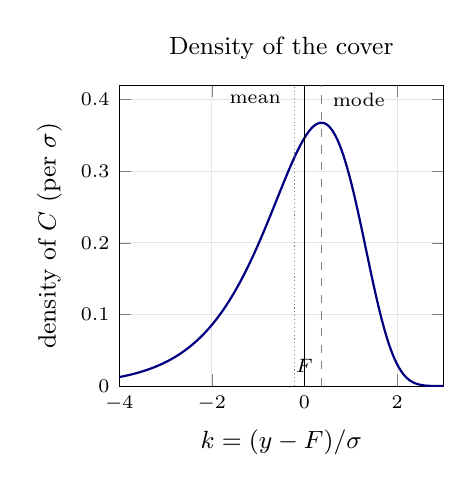
\begin{tikzpicture}
\begin{axis}[
  width=0.47\textwidth,height=5.4cm,
  xlabel={$k=(y-F)/\sigma$},
  ylabel={density of $C$ (per $\sigma$)},
  xmin=-4,xmax=3,ymin=0,ymax=0.42,
  grid=major,grid style={gray!20},
  samples=200,domain=-4:3,
  title={\small Density of the cover},
  tick label style={font=\scriptsize},label style={font=\small}]
\addplot[thick,NavyBlue] {exp(x-0.36651)*exp(-exp(x-0.36651))};
\addplot[gray,densely dotted] coordinates {(-0.2107,0) (-0.2107,0.42)};
\addplot[black,thin] coordinates {(0,0) (0,0.42)};
\addplot[gray,dashed] coordinates {(0.3665,0) (0.3665,0.42)};
\node[font=\scriptsize,anchor=east] at (axis cs:-0.3,0.40) {mean};
\node[font=\scriptsize,anchor=west] at (axis cs:0.40,0.40) {mode};
\node[font=\scriptsize,anchor=south] at (axis cs:0,0.005) {$F$};
\end{axis}
\end{tikzpicture}\hfill
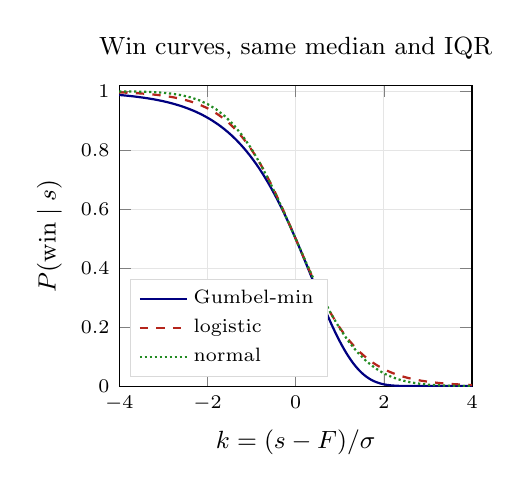
\begin{tikzpicture}
\begin{axis}[
  width=0.50\textwidth,height=5.4cm,
  xlabel={$k=(s-F)/\sigma$},
  ylabel={$P(\text{win}\mid s)$},
  xmin=-4,xmax=4,ymin=0,ymax=1.02,
  grid=major,grid style={gray!20},
  samples=161,domain=-4:4,
  title={\small Win curves, same median and IQR},
  legend style={at={(0.03,0.03)},anchor=south west,font=\scriptsize,draw=gray!30,fill=white},
  legend cell align=left,
  tick label style={font=\scriptsize},label style={font=\small}]
\addplot[thick,NavyBlue] {exp(-ln(2)*exp(x))};
\addlegendentry{Gumbel-min}
\addplot[thick,BrickRed,dashed] {1/(1+exp(x/0.71569))};
\addlegendentry{logistic}
\addplot[thick,ForestGreen,densely dotted] coordinates {(-4.00,0.9997) (-3.80,0.9994) (-3.60,0.9990) (-3.40,0.9982) (-3.20,0.9970) (-3.00,0.9950) (-2.80,0.9918) (-2.60,0.9871) (-2.40,0.9802) (-2.20,0.9704) (-2.00,0.9569) (-1.80,0.9387) (-1.60,0.9151) (-1.40,0.8851) (-1.20,0.8484) (-1.00,0.8045) (-0.80,0.7537) (-0.60,0.6966) (-0.40,0.6343) (-0.20,0.5681) (0.00,0.5000) (0.20,0.4319) (0.40,0.3657) (0.60,0.3034) (0.80,0.2463) (1.00,0.1955) (1.20,0.1516) (1.40,0.1149) (1.60,0.0849) (1.80,0.0613) (2.00,0.0431) (2.20,0.0296) (2.40,0.0198) (2.60,0.0129) (2.80,0.0082) (3.00,0.0050) (3.20,0.0030) (3.40,0.0018) (3.60,0.0010) (3.80,0.0006) (4.00,0.0003)};
\addlegendentry{normal}
\end{axis}
\end{tikzpicture}
\caption{Left: density of the cover in units of $\sigma$ from fair. Right: win curves of three laws calibrated to the same median and interquartile range. At $k=+2$ the Gumbel-min curve wins 0.6\% against 5.8\% (logistic) and 4.3\% (normal); at $k=-2$ it wins 91.0\% against 94.2\% and 95.7\%. Slopes at the median are almost identical, so the three laws differ only in what they say about tails, and the tails are exactly where censored records carry information.}
\label{fig:shape}
\end{figure}

\subsubsection{Closure under minima}
\begin{proposition}[Min-stability and independence of winner and level]\label{prop:minstable}
Let $Q_1,\dots,Q_N$ be independent, $Q_j$ Gumbel-min with median $F_j$ and common scale $\sigma$. Then
\begin{enumerate}[label=(\roman*),itemsep=1pt]
\item $\min_jQ_j$ is Gumbel-min with scale $\sigma$ and median $F_{\min}=-\sigma\ln\sum_j e^{-F_j/\sigma}$ (a soft-minimum);
\item $\Prob(\arg\min_jQ_j=k)=e^{-F_k/\sigma}\big/\sum_je^{-F_j/\sigma}$;
\item $\arg\min_jQ_j$ is independent of $\min_jQ_j$.
\end{enumerate}
In particular, $N$ i.i.d.\ quotes with median $F^Q$ have a minimum with median $F^Q-\sigma\ln N$.
\end{proposition}
\begin{proof}
Write $\Lambda_j(y)=\ln2\cdot e^{(y-F_j)/\sigma}=e^{y/\sigma}\,\ln2\cdot e^{-F_j/\sigma}$. (i) $\Prob(\min_jQ_j>y)=\exp(-\sum_j\Lambda_j(y))=\exp\bigl(-e^{y/\sigma}\ln2\sum_je^{-F_j/\sigma}\bigr)$, which is of the form \eqref{eq:cumhaz} with the stated median. (ii)--(iii) The joint law of winner and level is
\[
\Prob(\arg\min=k,\ \min\in dy)=f_k(y)\prod_{j\ne k}S_j(y)\,dy=\lambda_k(y)\,e^{-\sum_j\Lambda_j(y)}\,dy,
\]
and $\lambda_k(y)/\sum_j\lambda_j(y)=e^{-F_k/\sigma}/\sum_je^{-F_j/\sigma}$ does not depend on $y$, so the joint density factorises.
\end{proof}

\subsubsection{Proportional hazards}
\begin{proposition}[Location family $=$ proportional hazards only for Gumbel-min]\label{prop:ph}
Let $S_0$ be a continuous survival function on $\R$ and consider the location family $S(y;F)=S_0(y-F)$. Its cumulative hazards are proportional, $\Lambda(y;F)=\Lambda(y;0)\,\psi(F)$ for all $y,F$, if and only if $S_0$ is Gumbel-min, in which case $\psi(F)=e^{-F/\sigma}$.
\end{proposition}
\begin{proof}
Write $\Lambda_0=-\ln S_0$. Proportionality reads $\Lambda_0(y-F)=\Lambda_0(y)\psi(F)$. Setting $y=F$ gives $\psi(F)=\Lambda_0(0)/\Lambda_0(F)$, hence $\Lambda_0(y-F)\Lambda_0(F)=\Lambda_0(y)\Lambda_0(0)$. With $\phi=\ln(\Lambda_0/\Lambda_0(0))$ and $u=y-F$ this is Cauchy's equation $\phi(u)+\phi(F)=\phi(u+F)$, whose continuous solutions are $\phi(u)=u/\sigma$ (with $\sigma>0$ because $\Lambda_0$ increases). So $\Lambda_0(u)=\Lambda_0(0)e^{u/\sigma}$, which is \eqref{eq:cumhaz}. The converse is immediate.
\end{proof}
Consequently, at a given scale, a multiplier $M$ on the fair charge, $F\to MF$, is equivalent to multiplying the hazard of losing at every charge level by $\exp(-(M-1)F/\sigma)$. Log-cumulative-hazard plots, $\ln(-\ln\hat S(y))$ against $y$, must be straight lines of slope $1/\sigma$; this is the main shape diagnostic (\S\ref{sec:validation}).

\subsubsection{Log-concavity}
\begin{proposition}[Concave record likelihoods]\label{prop:logconcave}
For fixed $\sigma$, each of the following is concave in the location $F$: $\ln S_C(y)$, $\ln f_C(y)$, $\ln(1-S_C(y))$ and $\ln\bigl(S_C(a)-S_C(b)\bigr)$ for $a<b$.
\end{proposition}
\begin{proof}
All four depend on $F$ through $z=(\cdot-F)/\sigma+\zm$, which is affine in $F$, so it suffices to check concavity in $z$. $\ln S=-e^{z}$ and $\ln f=z-e^{z}-\ln\sigma$ are concave. The SEV density is log-concave; by Prékopa's theorem its distribution function, its survival function and its integral over any interval of fixed length are log-concave in the shift, which covers the last two terms.
\end{proof}
Concavity holds in $F$, not in $\eta=\ln F$; with the log link of Section~\ref{sec:location} the daily objective is not globally concave, which is why the fit is warm-started and the intraday Newton step uses a curvature floor (\S\ref{sec:intraday}). Mixture terms (\S\ref{sec:datamap}, \S\ref{sec:limitations}) also break concavity.

\subsubsection{Scale proportional to level: a universal relative curve}
With the scale specification of Section~\ref{sec:scale}, $\sigma_i=\kappa_iF_i$ where $\kappa_i=\kappa_0e^{\bm\xi\T\bm w_i}$ depends only on market-state covariates, not on bond, client or size. Substituting in \eqref{eq:S},
\begin{equation}\label{eq:relative}
\Prob(\text{win}\mid s)=2^{-\exp\left((s/F_i-1)/\kappa_i\right)} .
\end{equation}
The win probability depends on the charge only through the ratio $s/F_i$. Quoting at $1.2\times$ fair wins the same fraction of trades for every bond, client and size in a given market state. This is the property that makes a purely multiplicative representation of the fair charge consistent: multipliers move $F_i$, and the shape of the curve in relative terms is set once by $\kappa_i$.

\subsubsection{The logistic curve as a special case}
\begin{proposition}[Gumbel cover plus non-price noise gives the logistic]\label{prop:logistic}
Suppose that the client perceives our quote as $s+\sigma(\varepsilon_0-\zm)$, where $\varepsilon_0\sim\mathrm{SEV}(0,1)$ is independent non-price noise (relationship, settlement, operational preference), and the cover is \eqref{eq:cover} with the same $\sigma$. Then
\[
\Prob(\text{win}\mid s)=\frac{1}{1+e^{(s-F)/\sigma}} .
\]
\end{proposition}
\begin{proof}
Proposition~\ref{prop:minstable}(ii) with two ``dealers'' of medians $s$ and $F$.
\end{proof}
We choose the deterministic-quote version \eqref{eq:S} as the baseline because we know exactly what we sent, and systematic client preferences are captured by client multipliers. The logistic remains a principled alternative with a clear interpretation, to be selected by out-of-sample log score.

%----------------------------------------------------------------------
\subsection{How the distribution fits our data representation}\label{sec:datamap}
%----------------------------------------------------------------------

\subsubsection{Every record is an interval}
For each traded inquiry we ask one question: \emph{given what we observed, between which two charges must the cover lie?} The answer is a pair of charges $(L_i,U_i)$, both in bp over the reference mid with the sign convention \eqref{eq:charge}:
\begin{itemize}[itemsep=1pt]
\item $L_i$ is the \textbf{lowest} value the cover can take given the record (the lower bound), possibly $-\infty$;
\item $U_i$ is the \textbf{highest} value the cover can take given the record (the upper bound), possibly $+\infty$.
\end{itemize}
The probability that the model assigns to the record is the probability that the cover falls between the two bounds. Since $S(L_i)$ is the probability that the cover is above $L_i$ and $S(U_i)$ the probability that it is above $U_i$, their difference is the probability that it lies in between:
\begin{equation}\label{eq:unified}
\Prob(L_i<C_i\le U_i)=S_C(L_i)-S_C(U_i),\qquad
\ell_i\;=\;\ln\bigl[S_C(L_i)-S_C(U_i)\bigr],
\end{equation}
with the conventions $S(-\infty)=1$ (the cover is surely above $-\infty$) and $S(+\infty)=0$. All record types then share this single formula; only the bounds differ (Table~\ref{tab:intervals}).
\begin{table}[h]
\centering
\begin{tabular}{lllll}
\toprule
Code & $L_i$ & $U_i$ & Fallback $(L'_i,U'_i)$, weight $\rho_i$ & Term \\
\midrule
$\Win$ & $s_i$ & $+\infty$ & --- & $-e^{z(s_i)}$ \\
$\Wc$ & $\max(c_i-\delta_i,s_i)$ & $c_i+\delta_i$ & $(s_i,+\infty)$ & interval \\
$\Dl$ & $c_i-\delta_i$ & $\min(c_i+\delta_i,s_i)$ & $(-\infty,s_i)$ & interval \\
$\Dn$ & $-\infty$ & $s_i$ & --- & $\lmexp\bigl(e^{z(s_i)}\bigr)$ \\
\bottomrule
\end{tabular}
\caption{Interval representation. $\delta_i$ is the half-width of a reported level (mid error, rounding, time between inquiry and print). $\rho_i$ is the probability that the reported level does not belong to this inquiry (tape mismatch); the record then falls back to the pure censoring information. $\Dcv$ is not an interval on $C$ and is handled separately (Appendix~\ref{app:orderstat}).}
\label{tab:intervals}
\end{table}
\paragraph{Reading the table.}
\begin{itemize}[itemsep=2pt]
\item \textbf{Won, no cover} ($\Win$): every competitor was worse than us, so the cover is above our charge: $L_i=s_i$, no upper bound. The term is $\ln S_C(s_i)$, the log-probability of winning at $s_i$.
\item \textbf{Lost, no level} ($\Dn$): someone beat us, so the cover is below our charge: no lower bound, $U_i=s_i$. The term is $\ln(1-S_C(s_i))$, the log-probability of losing at $s_i$.
\item \textbf{Lost, tape level $c_i$} ($\Dl$): the cover is close to $c_i$, within the uncertainty $\pm\delta_i$ of the reported level, and it must also be below our charge since we lost; hence the upper bound $\min(c_i+\delta_i,s_i)$.
\item \textbf{Won, cover $c_i$ disclosed} ($\Wc$): the cover is close to $c_i$ and must also be above our charge since we won; hence the lower bound $\max(c_i-\delta_i,s_i)$.
\end{itemize}
The clipping by $s_i$ in the last two rows ensures that the record never contradicts its own outcome, even when the reported level is noisy.

\paragraph{Worked example.} We quote $s_i=3.0$\,bp, with $\delta_i=0.3$\,bp for any reported level.
\begin{center}
\small
\begin{tabular}{llll}
\toprule
Outcome & $L_i$ & $U_i$ & Contribution $\ell_i$ \\
\midrule
won, no cover & $3.0$ & $+\infty$ & $\ln\Prob(C_i>3.0)$ \\
won, cover disclosed at $3.4$ & $3.1$ & $3.7$ & $\ln\Prob(3.1<C_i\le3.7)$ \\
lost, tape at $2.2$ & $1.9$ & $2.5$ & $\ln\Prob(1.9<C_i\le2.5)$ \\
lost, tape at $2.9$ & $2.6$ & $3.0$ & $\ln\Prob(2.6<C_i\le3.0)$ \\
lost, no level & $-\infty$ & $3.0$ & $\ln\Prob(C_i\le3.0)$ \\
\bottomrule
\end{tabular}
\end{center}
In the fourth row the interval $2.9\pm0.3$ is cut at $3.0$, because a cover above our charge would have meant a win. As $\delta_i\to0$ the interval shrinks to the point $c_i$ and $\ell_i$ becomes the log-density at $c_i$ plus a constant; this limit is used numerically for very narrow intervals (\S\ref{sec:datamap}, Numerics).

\paragraph{Uncertain tape match.} A matched print may belong to another trade. With probability $\rho_i$ we therefore fall back to the information carried by the outcome alone, the interval $(L'_i,U'_i)=(s_i,+\infty)$ for a win or $(-\infty,s_i)$ for a loss. The general record contribution is
\begin{equation}\label{eq:mixture}
\ell_i=\ln\Bigl\{(1-\rho_i)\bigl[S_C(L_i)-S_C(U_i)\bigr]+\rho_i\bigl[S_C(L'_i)-S_C(U'_i)\bigr]\Bigr\}.
\end{equation}

\begin{figure}[h]
\centering
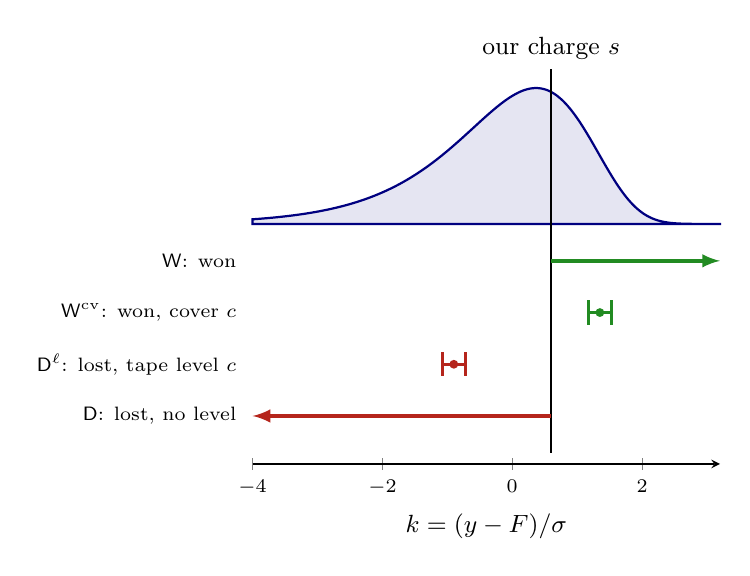
\begin{tikzpicture}
\begin{axis}[
  width=0.62\textwidth,height=6.6cm,
  xmin=-4,xmax=3.2,ymin=-0.65,ymax=0.42,
  axis x line=bottom, axis y line=none,
  xlabel={$k=(y-F)/\sigma$},
  samples=200,domain=-4:3.2,
  tick label style={font=\scriptsize},label style={font=\small},
  clip=false]
\addplot[thick,NavyBlue,fill=NavyBlue!10] {exp(x-0.36651)*exp(-exp(x-0.36651))} \closedcycle;
\addplot[black,thick] coordinates {(0.6,-0.62) (0.6,0.42)};
\node[font=\small,anchor=south] at (axis cs:0.6,0.42) {our charge $s$};
\draw[very thick,ForestGreen,-latex] (axis cs:0.6,-0.10) -- (axis cs:3.2,-0.10);
\node[font=\scriptsize,anchor=east] at (axis cs:-4.1,-0.10) {$\Win$: won};
\draw[very thick,ForestGreen,|-|] (axis cs:1.15,-0.24) -- (axis cs:1.55,-0.24);
\fill[ForestGreen] (axis cs:1.35,-0.24) circle (1.6pt);
\node[font=\scriptsize,anchor=east] at (axis cs:-4.1,-0.24) {$\Wc$: won, cover $c$};
\draw[very thick,BrickRed,|-|] (axis cs:-1.1,-0.38) -- (axis cs:-0.7,-0.38);
\fill[BrickRed] (axis cs:-0.9,-0.38) circle (1.6pt);
\node[font=\scriptsize,anchor=east] at (axis cs:-4.1,-0.38) {$\Dl$: lost, tape level $c$};
\draw[very thick,BrickRed,latex-] (axis cs:-4,-0.52) -- (axis cs:0.6,-0.52);
\node[font=\scriptsize,anchor=east] at (axis cs:-4.1,-0.52) {$\Dn$: lost, no level};
\end{axis}
\end{tikzpicture}
\caption{Each record restricts the cover to an interval; its likelihood is the probability mass of the density of $C$ over that interval. Wins (green) lie to the right of $s$, losses (red) to the left. Reported levels are short intervals of half-width $\delta$.}
\label{fig:intervals}
\end{figure}

\subsubsection{What each record identifies}
\begin{itemize}[itemsep=2pt]
\item \textbf{Wins without cover} bound $C_i$ from below. Because the right tail is double-exponential, a win at a charge well above $F_i$ is very surprising ($-\ln S$ grows like $e^{k}$): such records push $F_i$ up strongly. Wins at or below fair carry little information.
\item \textbf{Losses without level} bound $C_i$ from above. The left tail is only exponential, so a loss at a tight charge is not very surprising: these records move $F_i$ down gently.
\item \textbf{Tape and cover levels} locate $C_i$ to within $\pm\delta_i$; they are the only records that identify the \emph{scale} directly.
\end{itemize}
\begin{decision}
\textbf{Identification of the scale depends on tape matching.} With flags only, the likelihood depends on $(s_i-F_i)/\sigma_i$; if traders always quote near fair, every record says ``about 50\%'' whatever $\sigma$, and the scale is weakly identified. Levels matched from the tape and disclosed covers measure the spread of $C$ directly. Because $\sigma_i=\kappa_iF_i$ with $\kappa_i$ shared by all bonds and clients, a moderate number of matched levels pins the scale for the entire universe.
\end{decision}

\subsubsection{Data layout}
The model consumes one row per resolved inquiry and two sparse design matrices.
\begin{center}
\small
\begin{tabularx}{\textwidth}{lX}
\toprule
Column & Content \\
\midrule
keys & inquiry id, $t_i$, bond, client, tier, venue, session, side, country, curve node $j(b)$ \\
size & $\ln(q_i/q^\star_b)$ \\
competition & $n_i$ (or missing) \\
quote & $s_i$ (bp) \\
interval & $L_i,U_i$; fallback $L'_i,U'_i$; $\rho_i$ (Table~\ref{tab:intervals}) \\
type & $\Win,\Wc,\Dl,\Dn,\Dcv,\NT$ \\
scale covariates & mid quality, volatility proxy, session dummies, $\ln n_i$ \\
weight & $w_i$ (time decay) \\
\bottomrule
\end{tabularx}
\end{center}
The location and scale are linear predictors on these rows:
\begin{equation}\label{eq:design}
\bm\eta=\bm X\btheta_{\mathrm{loc}},\qquad \ln\bm\sigma=\bm\eta+\ln\kappa_0+\bm W\bm\xi,
\end{equation}
where each row of $\bm X$ has one-hot entries for the curve node, bond, tier, client, venue, session and side, and B-spline weights for the size curve (Section~\ref{sec:location}). $\bm X$ has about ten non-zeros per row regardless of the size of the universe, so the gradient and Hessian of the objective are cheap sparse products.

\subsubsection{Numerics}
All terms are computed on the log scale with $w=e^{z}$:
\[
\ln S(y)=-w,\qquad \ln(1-S(y))=\lmexp(w),\qquad \ln\bigl(S(L)-S(U)\bigr)=-w_L+\lmexp(w_U-w_L),
\]
where $\lmexp(x)=\ln(1-e^{-x})$ is evaluated as $\ln(-\mathrm{expm1}(-x))$ for $x\le\ln2$ and $\mathrm{log1p}(-e^{-x})$ otherwise. When $U_i-L_i<10^{-3}\sigma_i$ the density form $\ln f_C(c_i)+\ln(U_i-L_i)$ is used instead.

%----------------------------------------------------------------------
\subsection{Limitations and safeguards}\label{sec:limitations}
%----------------------------------------------------------------------
\begin{description}[itemsep=3pt,leftmargin=0pt]
\item[Thin right tail and non-price wins.] Some wins have nothing to do with price: a client who always gives us the ticket, an allocation, a mis-hit. A win at $k=+3$ costs $\ln2\cdot e^{3}\approx 13.9$ nats against $4.2$ under a logistic with the same median and IQR, so a few such records can drag a client's fair charge upward. Safeguard: in the likelihood of flag-only records, replace $S_C$ by the contaminated curve
\[
\tilde S(y)=\epsilon_W+(1-\epsilon_W-\epsilon_L)\,S_C(y),
\]
with small fixed $\epsilon_W,\epsilon_L$ (e.g.\ 1\%, per tier if needed). This is a mixture handled by the formulas of Appendix~\ref{app:derivatives}. Quotes are always computed with the uncontaminated $S_C$: the contamination is a robustness device for estimation, and a curve with $\epsilon_W>0$ would make arbitrarily wide quotes look profitable.
\item[Small dealer counts.] The extreme-value argument (a) is asymptotic; with two or three dealers the true cover may be less skewed. The log-cumulative-hazard diagnostic detects this; if it fails systematically for small $n_i$, let the scale depend on $\ln n_i$ (already in $\bm w_i$) or switch to the logistic for those venues.
\item[Common scale.] Closure under minima, the dealer-count adjustment and the reservation model need competitors (and the client limit) to share $\sigma_i$. The baseline model only needs the cover's own scale, so the assumption matters only once those extensions are switched on.
\item[Mid noise.] A Gumbel variable plus Gaussian mid error is no longer Gumbel. We do not convolve; mid uncertainty enters through the interval half-widths $\delta_i$ and through mid-quality covariates in the scale.
\end{description}

%----------------------------------------------------------------------
\subsection{Alternatives considered}\label{sec:alternatives}
%----------------------------------------------------------------------
\begin{table}[h]
\centering
\small
\begin{tabular}{lccccc}
\toprule
 & Gumbel-min & Logistic & Normal & Student-$t$ & Nonparametric \\
\midrule
Closed-form $S$ and $\ln S$ & yes & yes & via $\Phi$ & no & empirical \\
Closed under minima & yes & no & no & no & --- \\
Winner independent of level & yes & no & no & no & --- \\
Log-concave (unique updates) & yes & yes & yes & no & --- \\
Proportional hazards & yes & no & no & no & Cox \\
Skewed like a best-of-$N$ & yes & no & no & no & any \\
Closed-form optimal quote & Lambert $W$ & Lambert $W$ & no & no & no \\
Robust to non-price wins & weak$^{*}$ & good & moderate & good & good \\
Pooling across cells & yes & yes & yes & yes & no \\
\bottomrule
\end{tabular}
\caption{Candidate laws for the cover. $^{*}$Mitigated by the contamination term of \S\ref{sec:limitations}. A nonparametric (Turnbull) estimator is used as a diagnostic, not as the model, because it cannot pool across bonds and clients.}
\label{tab:alternatives}
\end{table}

%----------------------------------------------------------------------
\subsection{Dealer count}\label{sec:dealers}
%----------------------------------------------------------------------
Under Assumption~\ref{ass:iid} with each $Q_{ij}$ Gumbel-min of median $F^Q_i$ and scale $\sigma_i$, Proposition~\ref{prop:minstable} gives
\begin{equation}\label{eq:dealers}
F_i \;=\; F^Q_i - \sigma_i\ln(n_i-1).
\end{equation}
When $n_i$ is observed, the multiplicative structure of Section~\ref{sec:location} is placed on the per-dealer charge $F^Q_i$, which is more stable across venues and protocols, and the street fair charge follows from \eqref{eq:dealers}. When $n_i$ is not observed, its effect is absorbed by the venue and client effects.

%======================================================================
\section{Structural model for location and scale}\label{sec:location}
%======================================================================

\subsection{Location: per-bond fair charge times multipliers}
Let $\eta_i=\ln F_i$ (or $\ln F^Q_i$ under \eqref{eq:dealers}). We impose the additive decomposition
\begin{equation}\label{eq:eta}
\eta_i \;=\; \underbrace{\eta^{\mathrm{bond}}_{b(i)}}_{\text{bond at }q^\star}
+ \underbrace{h\bigl(\ln(q_i/q^\star_{b})\bigr)}_{\text{size curve}}
+ \alpha_{k(i)} + u_{c(i)} + \nu_{v(i)} + \delta\,d_i + \omega_{p(i)},
\end{equation}
with the bond term made of a country curve evaluated at the bond's maturity and an idiosyncratic spread,
\begin{equation}\label{eq:bond}
\eta^{\mathrm{bond}}_b \;=\; \beta_0 + f_{g(b)}(T_b) + e_b .
\end{equation}
Here $f_g$ is the maturity curve of country $g$ (\S\ref{sec:curve}), $e_b$ the idiosyncratic bond spread, $h$ the size curve, $\alpha_k$ the tier effect, $u_c$ the client deviation from its tier, $\nu_v$ the venue effect, $\delta$ half the bid/offer asymmetry and $\omega_p$ the trading-session effect (\S\ref{sec:session}).

Exponentiating gives the multiplicative reading:
\begin{equation}\label{eq:multiplicative}
\boxed{\;
F_i \;=\; F^{0}_{b}\cdot S(q_i)\cdot M^{\mathrm{tier}}_{k}\cdot M^{\mathrm{cl}}_{c}\cdot M^{\mathrm{ven}}_{v}\cdot M^{\mathrm{side}}_{d}\cdot M^{\mathrm{ses}}_{p},
\qquad
F^0_b=\underbrace{e^{\beta_0+f_{g(b)}(T_b)}}_{\text{country curve}}\cdot\underbrace{e^{e_b}}_{\text{idiosyncratic}}
\;}
\end{equation}
with $S(q)=e^{h(\ln(q/q^\star_b))}$, $M^{\mathrm{tier}}_k=e^{\alpha_k}$, $M^{\mathrm{cl}}_c=e^{u_c}$, $M^{\mathrm{ven}}_v=e^{\nu_v}$, $M^{\mathrm{side}}_d=e^{\delta d}$, $M^{\mathrm{ses}}_p=e^{\omega_p}$.

\begin{decision}
\textbf{No liquidity score, no age.} Bond characteristics such as liquidity, age, benchmark or on-the-run status, issue size and repo specialness are not modelled as covariates. Their persistent effect on the charge is absorbed by $e_b$, estimated from the bond's own inquiry history. Consequences:
\begin{enumerate}[itemsep=1pt,label=(\alph*)]
\item the model has no dependency on an external liquidity score or on feature engineering;
\item a bond with little history is priced close to its country curve, because $e_b$ is shrunk toward zero; a bond with a rich history gets its own spread;
\item slow changes (ageing, loss of benchmark status) are tracked with a lag of the order of the time-decay half-life $H$ of the daily fit, and faster within the day by the intraday filter, where $e_b$ is a state.
\end{enumerate}
\end{decision}

\subsection{Country maturity curve}\label{sec:curve}

\paragraph{Nodes.} For country $g$, take all bonds of the tradeable universe (not only those with inquiries) and sort their maturities. Maturities closer than a tolerance $\Delta_{\min}$ (e.g.\ two weeks) are merged into one node. This gives nodes $\tau_{g,1}<\dots<\tau_{g,J_g}$ and a map $b\mapsto j(b)$. The curve is represented by its node values,
\[
\bff_g=(f_{g,1},\dots,f_{g,J_g})\T,\qquad f_{g(b)}(T_b)=f_{g,j(b)} .
\]
The argument is time to maturity in years, as in current desk practice; a transformed argument such as $\ln(1+T)$ (which stretches the short end) is a drop-in replacement.

\paragraph{Curvature penalty between consecutive maturities.} For interior nodes $j=2,\dots,J_g-1$, with gaps $\Delta_j=\tau_{g,j}-\tau_{g,j-1}$, the second divided difference is
\begin{equation}\label{eq:divdiff}
D_{g,j}\;=\;\frac{2}{\Delta_j+\Delta_{j+1}}\left(\frac{f_{g,j+1}-f_{g,j}}{\Delta_{j+1}}-\frac{f_{g,j}-f_{g,j-1}}{\Delta_j}\right),
\end{equation}
an estimate of $f_g''$ at $\tau_{g,j}$ that is exact for quadratics and valid for unequally spaced maturities. The penalty is
\begin{equation}\label{eq:curvpen}
\mathrm{pen}_g(\bff_g)=\frac{\lambda_g}{2}\sum_{j=2}^{J_g-1}\frac{\Delta_j+\Delta_{j+1}}{2}\,D_{g,j}^2=\frac{\lambda_g}{2}\,\bff_g\T\bm K_g\bff_g,\qquad \bm K_g=\bm D_g\T\bm H_g\bm D_g,
\end{equation}
where $\bm D_g$ is the $(J_g-2)\times J_g$ matrix of \eqref{eq:divdiff} and $\bm H_g$ the diagonal matrix of trapezoid weights (Appendix~\ref{app:curve}). The weighted sum approximates $\int f_g''(\tau)^2d\tau$, so the penalty does not depend on how densely a country issues.

\paragraph{Probabilistic reading.} \eqref{eq:curvpen} is the negative log-density of a Gaussian prior with precision $\lambda_g\bm K_g$: a second-order intrinsic Gaussian Markov random field, the discrete counterpart of an integrated Wiener process. Its posterior mean, given node data, is a cubic smoothing spline through the nodes. Two consequences matter here:
\begin{itemize}[itemsep=1pt]
\item a node with no inquiries (a bond never asked) receives its value by smooth interpolation from its neighbours, so every bond in the universe has a fair charge from day one;
\item $\bm K_g$ has rank $J_g-2$: its null space is the straight lines $a+b\tau$, which the penalty leaves free.
\end{itemize}

\paragraph{Level and slope.} We decompose
\begin{equation}\label{eq:levelslope}
f_{g,j}=a_g+b_g\,(\tau_{g,j}-\tau_{\mathrm{ref}})+\tilde f_{g,j},\qquad \sum_j\tilde f_{g,j}=\sum_j\tilde f_{g,j}\tau_{g,j}=0,
\end{equation}
with $\tau_{\mathrm{ref}}$ a reference maturity common to all countries (e.g.\ 10 years). The level and slope are pooled across countries,
\[
a_g\sim\mathcal N(0,\tau_a^2),\qquad b_g\sim\mathcal N(\bar b,\tau_b^2),
\]
so that a country with only a few bonds borrows its slope from the others. $e^{a_g}$ is reported as the \textbf{country multiplier}: the fair charge of a country relative to $e^{\beta_0}$ at the reference maturity. For countries with fewer than three nodes $\tilde{\bff}_g$ is empty and the curve is a line.

\paragraph{Curve versus idiosyncratic spread.} With $e_b\sim\mathcal N(0,\tau_e^2)$, the split of a bond's deviation between the curve and its own spread is governed by $\lambda_g$ and $\tau_e$. A large $\lambda_g$ forces the curve toward a line and pushes deviations into $e_b$; a small $\lambda_g$ lets the curve follow individual bonds, and $e_b$ is then only identified where several bonds share a node or where the curve is constrained by neighbours. $\lambda_g$ is a desk-level choice of how smooth a country should be; the current desk value is the natural starting point, with weekly re-tuning by marginal likelihood (\S\ref{sec:daily}).

\subsection{Size curve}
$h$ is a cubic B-spline in $\ln(q/q^\star_b)$ with $h(0)=0$, a second-difference smoothness penalty, and an optional monotonicity constraint above $q^\star_b$ (larger blocks cost more). Below $q^\star_b$ the curve is left free, which accommodates odd-lot premia. One curve is shared by all bonds; if diagnostics show that the size effect differs by country, use per-country curves $h_g$ pooled toward the common one.

\subsection{Trading session}\label{sec:session}
The time of day enters only through a three-level session factor. With $t_i$ the RFQ receipt time in London local time (so boundaries follow daylight-saving changes),
\begin{equation}\label{eq:session}
p(i)=\begin{cases}
\mathrm{pre} & t_i<\text{08:15},\\
\mathrm{core} & \text{08:15}\le t_i<\text{16:30},\\
\mathrm{post} & t_i\ge\text{16:30},
\end{cases}
\qquad \omega_{\mathrm{core}}=0 .
\end{equation}
$M^{\mathrm{ses}}_{\mathrm{pre}}=e^{\omega_{\mathrm{pre}}}$ and $M^{\mathrm{ses}}_{\mathrm{post}}=e^{\omega_{\mathrm{post}}}$ are the charges outside core hours relative to the same inquiry inside them. Session dummies are also included in the scale covariates (\S\ref{sec:scale}), so the win curve is both shifted and flattened off-hours. If diagnostics ask for it, session effects by country, $\omega_{p,g}\sim\mathcal N(\omega_p,\tau_\omega^2)$, can be added.

\begin{decision}
\textbf{Sessions are static intraday.} $\omega_p$ is estimated in the morning fit and is not part of the intraday state. Its effect enters each inquiry through the morning predictor $\eta^0_i$, so the filter states are expressed in core-session units and an observation in any session updates them coherently.
\end{decision}

\subsection{Scale}\label{sec:scale}
We let the dispersion scale with the level:
\begin{equation}\label{eq:scale}
\ln\sigma_i \;=\; \eta_i + \ln\kappa_0 + \bm{\xi}\T\bm{w}_i,
\end{equation}
so that $\sigma_i/F_i=\kappa_i=\kappa_0e^{\bm\xi\T\bm w_i}$, with $\bm w_i$ containing: mid quality (staleness, number of contributing sources), the session dummies $\one\{p(i)=\mathrm{pre}\}$ and $\one\{p(i)=\mathrm{post}\}$, a volatility proxy (index or futures intraday range) and $\ln n_i$. $\bm w_i$ deliberately excludes bond, client and size identifiers, which gives the universal relative curve \eqref{eq:relative}.

\begin{remark}[Negative charges]
If a non-trivial fraction of covers lies through mid in some country, use an affine reparameterisation $F_i=\phi_g+e^{\eta_i}$ with a fixed floor $\phi_g\le 0$ per country. Multipliers then act on $F_i-\phi_g$. Covers below zero are already allowed by \eqref{eq:cover}; the floor only matters if the median itself can be negative.
\end{remark}

\subsection{Priors and identifiability}
\begin{center}
\small
\begin{tabular}{lll}
\toprule
Block & Prior / constraint & Role \\
\midrule
$\beta_0,\bm\xi,\ln\kappa_0,\delta,\bar b$ & weak $\mathcal N(0,10^2)$ & fixed effects \\
$a_g$ & $\mathcal N(0,\tau_a^2)$ & country level, pooled \\
$b_g$ & $\mathcal N(\bar b,\tau_b^2)$ & country slope, pooled \\
$\tilde{\bff}_g$ & curvature penalty $\lambda_g\bm K_g$, orthogonal to lines & country curve shape \\
$e_b$ & $\mathcal N(0,\tau_e^2)$ & idiosyncratic bond spread \\
$\alpha_k$ & $\alpha_{k_0}=0$ (reference tier) & tier multiplier \\
$u_c$ & $\mathcal N(0,\tau^2_{u,k(c)})$ & client, pooled toward its tier \\
$\nu_v$ & $\nu_{v_0}=0$ (reference venue) & venue multiplier \\
$\omega_p$ & $\omega_{\mathrm{core}}=0$ (reference session) & session multiplier \\
spline $h$ & 2nd-difference penalty; $h(0)=0$ & size curve \\
\bottomrule
\end{tabular}
\end{center}
With these constraints, $F^0_b$ is the median cover for bond $b$ at size $q^\star_b$, for an average client of the reference tier, on the reference venue, averaged over sides, in the core session.

%======================================================================
\section{Reservation and trade propensity}\label{sec:reservation}
%======================================================================

We allow two kinds of client behaviour, mixed per inquiry:
\begin{itemize}[itemsep=1pt]
\item with probability $1-\pi_i$ the inquiry is price discovery, $R_i=-\infty$;
\item with probability $\pi_i$ the client has a reservation $R_i$, Gumbel-min with median $F^R_i$ and the \emph{same} scale $\sigma_i$ as $C_i$.
\end{itemize}
$\operatorname{logit}\pi_i$ and $F^R_i=F_i+\Delta_{k(i)}$ are modelled with client-tier random effects.

\begin{proposition}[Outcome probabilities]\label{prop:outcomes}
Under Assumptions~\ref{ass:censoring}--\ref{ass:indep} and the common scale, $Y_i=\min(C_i,R_i)$ is Gumbel-min with scale $\sigma_i$ and median
\[
F^Y_i=-\sigma_i\ln\!\bigl(e^{-F_i/\sigma_i}+e^{-F^R_i/\sigma_i}\bigr),
\qquad
p^C_i=\frac{1}{1+e^{(F_i-F^R_i)/\sigma_i}},\quad p^R_i=1-p^C_i .
\]
Writing $S_Y,f_Y$ for its survival and density and $F_Y=1-S_Y$,
\begin{align*}
\Prob(\Win) &= \pi_i\,S_Y(s_i), &
\Prob(\Wc,\,C_i\in dc) &= \pi_i\,f_C(c)\,S_R(s_i)\,dc,\quad c>s_i,\\
\Prob(\Dl,\,C_i\in dc) &= \pi_i\,p^C_i\,f_Y(c)\,dc,\quad c<s_i, &
\Prob(\Dn) &= \pi_i\,p^C_i\,F_Y(s_i),\\
\Prob(\NT) &= (1-\pi_i)+\pi_i\,p^R_i\,F_Y(s_i). &&
\end{align*}
\end{proposition}
\begin{proof}
Direct application of Proposition~\ref{prop:minstable} with two ``competitors'', $C_i$ and $R_i$: $Y_i$ is their minimum, $p^C_i$ the probability that the minimum is $C_i$, and the identity of the minimum is independent of its value. The probabilities sum to one.
\end{proof}

\begin{decision}
\textbf{Baseline: no binding reservation} ($F^R_i=+\infty$, so $p^C_i=1$, $Y_i=C_i$). Then $\NT$ inquiries only inform $\pi_i$, which is fitted as a separate logistic model, and the cover likelihood uses traded inquiries only. The full reservation model is switched on per tier once enough $\NT$ data with variation in $s_i$ exist; $\pi_i$ and $F^R_i$ are only weakly separately identified, so $\pi_i$ should then be fixed or strongly regularised.
\end{decision}

%======================================================================
\section{Likelihood}
%======================================================================

\subsection{Per-inquiry contributions}
Under the baseline, conditional on the inquiry trading, each record contributes the interval term \eqref{eq:unified}, with the fallback mixture \eqref{eq:mixture} for reported levels and, for flag-only records, the contaminated curve of \S\ref{sec:limitations}:
\begin{align}
\ell_i^{\Win} &= \ln\tilde S(s_i), \label{eq:lW}\\
\ell_i^{\Wc},\ \ell_i^{\Dl} &= \text{\eqref{eq:mixture} with the intervals of Table~\ref{tab:intervals}}, \label{eq:lWc}\\
\ell_i^{\Dn} &= \ln\bigl[1-\tilde S(s_i)\bigr], \label{eq:lD}\\
\ell_i^{\Dcv} &= \ln\Bigl[(n_i-1)\,F_Q(s_i)\,S_Q(s_i)^{n_i-2}\Bigr],\quad S_Q=S_C^{1/(n_i-1)}\quad\text{(Assumption~\ref{ass:iid})}. \label{eq:lcv}
\end{align}
The interval half-width is $\delta_i=c_\delta\,\sigma^{\mathrm{mid}}_i+c_t\sqrt{|\tau_i-t_i|}\,\mathrm{vol}_i$, a multiple of the mid uncertainty plus a timing term. The tape-match probability $\rho_i$ comes from a match-quality score on size, side, time gap and number of candidate prints. The trade-propensity model contributes $\ln\pi_i$ for traded inquiries and $\ln(1-\pi_i)$ for $\NT$; under the full reservation model the terms of Proposition~\ref{prop:outcomes} replace these.

\subsection{Total objective}
With exponential time-decay weights $w_i=2^{-(T-t_i)/H}$ (half-life $H$, in business days), the daily objective is the weighted log-posterior
\begin{multline}\label{eq:objective}
\mathcal{J}(\btheta)\;=\;\sum_{i}w_i\,\ell_i(\btheta)
\;-\;\sum_g\Bigl[\frac{\lambda_g}{2}\,\tilde{\bff}_g\T\bm K_g\tilde{\bff}_g+\frac{a_g^2}{2\tau_a^2}+\frac{(b_g-\bar b)^2}{2\tau_b^2}\Bigr]
\;-\;\sum_b\frac{e_b^2}{2\tau_e^2}\\
\;-\;\sum_c\frac{u_c^2}{2\tau_{u,k(c)}^2}\;-\;\mathrm{pen}(h)\;-\;\tfrac12\|\bm\vartheta\|^2_{\mathrm{weak}},
\end{multline}
where $\btheta$ collects all parameters and $\bm\vartheta$ the fixed effects.

\subsection{Gradients}
Every term depends on $\btheta$ only through $(\eta_i,\ln\sigma_i)$, and through these only via the standardised levels $z_i(y)$ of \eqref{eq:z}. Appendix~\ref{app:derivatives} lists $\partial\ell/\partial z$ and $\partial^2\ell/\partial z^2$ for each type. The chain rule uses
\[
\frac{\partial z_i(y)}{\partial F_i}=-\frac1{\sigma_i},\qquad
\frac{\partial z_i(y)}{\partial\ln\sigma_i}=-\bigl(z_i(y)-\zm\bigr),
\]
and, because $\eta_i$ and $\ln\sigma_i$ are linear in the parameters \eqref{eq:design}, the gradient in $\btheta$ is a sparse product $\bm X\T(\cdot)$. In practice the objective is written once in an autodiff framework (JAX or PyTorch), with the closed forms used for testing and for the intraday filter.

%======================================================================
\section{Daily calibration}\label{sec:daily}
%======================================================================

\subsection{Procedure}
\begin{algorithm}[h]
\caption{Morning calibration (completed before the first pre-08:15 inquiry)}\label{alg:daily}
\begin{algorithmic}[1]
\State Build today's country nodes from the universe's maturities (merge within $\Delta_{\min}$); compute $\bm K_g$; map bonds to nodes.
\State Assemble inquiries over the last $3H$ business days; map quotes, covers and tape prints to charges via \eqref{eq:charge}--\eqref{eq:tape}.
\State Match losses to tape prints; compute $c_i,\delta_i,\rho_i$; build the interval table (Table~\ref{tab:intervals}).
\State Warm-start $\btheta$ from yesterday's estimate, mapping curve values by bond (nodes move as maturities roll); new bonds start on the interpolated curve with $e_b=0$, new clients at $u_c=0$.
\State Maximise $\mathcal J(\btheta)$ with L-BFGS (hyperparameters fixed).
\State Compute the Hessian $\bm H=-\nabla^2\mathcal J$ at the optimum (sparse); Laplace posterior $\btheta\sim\mathcal N(\hat\btheta,\bm H^{-1})$.
\State Extract marginal variances of reported quantities and the covariance block of the intraday state by sparse selected inversion.
\State Fit $\pi_i$ (logistic, tier and client random effects) on all inquiries.
\State Publish outputs (Table~\ref{tab:outputs}); run diagnostics (Section~\ref{sec:validation}).
\end{algorithmic}
\end{algorithm}

\textbf{Hyperparameters.} $\lambda_g,\tau_a,\tau_b,\tau_e,\tau_u$, the size-spline penalty and $H$ are re-tuned weekly, not daily, by maximising the Laplace approximation of the marginal likelihood or, more robustly, the out-of-sample predictive log score on the most recent week. $\lambda_g$ can also be held at the current desk value.

\begin{remark}[Daily step as a filter]
Instead of a rolling window, the morning fit can use yesterday's posterior, inflated by an overnight process noise, as the prior. The daily and intraday procedures are then the same filter run on two clocks. The rolling window is simpler to audit and is the recommended starting point.
\end{remark}

\subsection{Outputs}
\begin{table}[h]
\centering
\small
\begin{tabular}{lll}
\toprule
Output & Definition & Uncertainty \\
\midrule
Fair charge per bond & $F^0_b=e^{\beta_0+f_{g(b)}(T_b)+e_b}$ at $q^\star_b$ & $\mathrm{sd}(\eta^{\mathrm{bond}}_b)$ (relative) \\
\quad of which country curve & $e^{\beta_0+f_{g}(T)}$, all maturities & pointwise band \\
\quad of which idiosyncratic & $e^{e_b}$ & credible interval \\
Country multipliers & $M^{\mathrm{cty}}_g=e^{a_g}$ (at $\tau_{\mathrm{ref}}$) & credible interval \\
Size curve & $S(q)=e^{h(\ln(q/q^\star_b))}$ & pointwise band \\
Tier multipliers & $M^{\mathrm{tier}}_k=e^{\alpha_k}$ & credible interval \\
Client multipliers & $M^{\mathrm{cl}}_c=e^{u_c}$; flagged if idiosyncratic & credible interval \\
Venue, side & $e^{\nu_v}$, $e^{\pm\delta}$ & credible interval \\
Session multipliers & $M^{\mathrm{ses}}_{\mathrm{pre}}$, $M^{\mathrm{ses}}_{\mathrm{post}}$ & credible interval \\
Relative width & $\kappa_i=\sigma_i/F_i$ by market state & --- \\
Trade propensity & $\pi$ by tier/client & --- \\
\bottomrule
\end{tabular}
\caption{Morning outputs. For any inquiry, $F_i$ is the product \eqref{eq:multiplicative} and the win curve is \eqref{eq:relative}.}
\label{tab:outputs}
\end{table}

A client is flagged as \emph{idiosyncratic} when it has at least $N_{\min}$ traded inquiries in the window, $|\hat u_c|/\mathrm{sd}(u_c)>2$, and $|\hat u_c|>\ln(1+\epsilon_M)$ for a materiality threshold $\epsilon_M$ (e.g.\ 15\%). Other clients are priced at their tier multiplier; shrinkage makes this automatic, the flag is for reporting. The same rule applied to $e_b$ flags bonds that trade persistently away from their country curve.

%======================================================================
\section{Intraday updating}\label{sec:intraday}
%======================================================================

\subsection{State}
The morning fit gives a linear predictor $\eta^0_i$ for any inquiry. Intraday we track deviations
\[
\bx_t=\bigl(\mu_t,\;a_{1,t},\dots,a_{G,t},\;\alpha_{1,t},\dots,\alpha_{K,t},\;(e_{b,t})_{b\in\mathcal B_t},\;(u_{c,t})_{c\in\mathcal C_t}\bigr),
\]
where $\mu_t$ is a market-wide factor, $a_{g,t}$ a parallel shift of country $g$'s curve, and $\mathcal B_t,\mathcal C_t$ are the bonds and clients seen so far today (components are added lazily, at their morning posterior). The inquiry's location is
\begin{equation}\label{eq:obs}
\eta_i(\bx)=\eta^0_i+\bh_i\T\bx,
\end{equation}
where $\bh_i$ has ones at the entries $\mu$, $a_{g(b(i))}$, $\alpha_{k(i)}$, $e_{b(i)}$, $u_{c(i)}$ and zeros elsewhere. The curve shape $\tilde{\bff}_g$, the size curve, the session and venue effects and the scales $\sigma_i$ are frozen at their morning values: they are second-order, noisier quantities, and freezing them keeps the update one-dimensional and stable.

\textbf{Dynamics.} Time is measured in hours from the first inquiry of the day; all three sessions use the same clock, the session effect being in $\eta^0_i$,
\begin{equation}\label{eq:dyn}
\bx_{t'}=\bx_t+\bm\zeta,\qquad \bm\zeta\sim\mathcal N\bigl(\bm0,\,\Qm\,(t'-t)\bigr),\qquad \Qm=\operatorname{diag}(q_\mu,q_a\bm1,q_\alpha\bm1,q_e\bm1,q_u\bm1).
\end{equation}
At the start of the day, $\bx_0\sim\mathcal N(\bm0,\Pm_0)$ with $\Pm_0$ the morning posterior covariance of the corresponding components (zero for $\mu$, plus an overnight variance).

\subsection{Rank-one Laplace update}
An inquiry is processed when its outcome is resolved, not when it arrives. Its likelihood depends on $\bx$ only through the scalar $r=\bh_i\T\bx$, the deviation of $\ln F_i$ from the morning value. Let $\bm m,\Pm$ be the predicted mean and covariance (after applying \eqref{eq:dyn} up to the update time), and
\[
r_0=\bh_i\T\bm m,\qquad v=\bh_i\T\Pm\bh_i .
\]
\textbf{Step 1 (scalar posterior).} Find the mode of $\ell_i(r)-(r-r_0)^2/(2v)$ by two or three Newton iterations from $r_0$:
\begin{equation}\label{eq:newton}
r\;\leftarrow\; r-\frac{(r-r_0)/v-g(r)}{1/v+H(r)},\qquad g=\frac{\partial\ell_i}{\partial r},\quad H=\max\Bigl(-\frac{\partial^2\ell_i}{\partial r^2},\,H_{\min}\Bigr),
\end{equation}
and set $\hat r$ to the result and $\hat v=(1/v+H(\hat r))^{-1}$. With $F_i=e^{\eta^0_i+r}$ and $\sigma_i$ frozen, $\vartheta_i:=F_i/\sigma_i$ and
\begin{equation}\label{eq:chain_r}
\frac{\partial z}{\partial r}=-\vartheta_i,\qquad \frac{\partial^2 z}{\partial r^2}=-\vartheta_i,
\qquad
g=-\vartheta_i\,\mathcal D\ell_i,\qquad -\frac{\partial^2\ell_i}{\partial r^2}=-\vartheta_i^2\,\mathcal D^2\ell_i+\vartheta_i\,\mathcal D\ell_i,
\end{equation}
where $\mathcal D$ is the derivative with respect to a common shift of all $z$-arguments of $\ell_i$ (Appendix~\ref{app:derivatives}). The floor $H_{\min}>0$ is needed because concavity in $F$ (Proposition~\ref{prop:logconcave}) does not imply concavity in $r=\ln F$.

\textbf{Step 2 (propagate to the state).} Treating the scalar posterior $\mathcal N(\hat r,\hat v)$ as the new information on $\bh_i\T\bx$ and conditioning the joint Gaussian,
\begin{equation}\label{eq:update}
\boxed{\;
\bm m\leftarrow\bm m+\Pm\bh_i\,\frac{\hat r-r_0}{v},\qquad
\Pm\leftarrow\Pm-\Pm\bh_i\bh_i\T\Pm\,\frac{v-\hat v}{v^2}.
\;}
\end{equation}
This is assumed-density filtering with a Laplace projection. The cost is $O(d^2)$ for a state of dimension $d$ (a few hundred at most).

\textbf{Reading the gain.} The vector $\Pm\bh_i/v$ splits the information among the components according to their current uncertainty: a first inquiry from a sparsely seen client mostly moves $u_c$; a stream of losses across many bonds of one country moves $a_g$; losses everywhere move $\mu$; repeated surprises on one bond move $e_b$. Off-diagonal terms created by earlier updates let a client observation also move the tier, and vice versa.

\subsection{Practicalities}
\begin{itemize}[itemsep=2pt]
\item \textbf{Delayed information.} A tape level often arrives after the outcome. Apply it when it arrives, with $v$ replaced by $v+\bh_i\T\Qm\bh_i\,(t_{\mathrm{now}}-t_i)$ to account for drift since $t_i$; if the earlier $\Dn$ update for the same inquiry was already applied, apply only the incremental information (difference of the $\Dl$ and $\Dn$ log-likelihoods).
\item \textbf{Robustness.} Cap $|\hat r-r_0|\le c_{\max}\sqrt v$; temper an observation ($\ell_i\to w\ell_i$, $w<1$) whose predictive tail probability is below $10^{-3}$, and log it.
\item \textbf{Process noise.} $\Qm$ is estimated by replaying historical days and maximising the one-step-ahead predictive log score $\sum_i\ln\int p(O_i\mid r)\,\mathcal N(r;r_0,v)\,dr$ (Gauss--Hermite, 10 nodes). A simple starting value is the variance of day-over-day changes of each morning estimate, divided by the length of the trading day.
\item \textbf{Reset.} Each morning the state is reset; the intraday deviations are not carried over, the morning fit absorbs them.
\end{itemize}

\subsection{Predictive win curve under parameter uncertainty}
For quoting, the plug-in curve $\pi_iS_C(s;r_0)$ understates uncertainty for sparse bonds and clients. The predictive curve
\begin{equation}\label{eq:predictive}
\bar p_i(s)=\pi_i\int S_C\bigl(s;\eta^0_i+r\bigr)\,\mathcal N(r;r_0,v)\,dr
\end{equation}
is flatter where $v$ is large and is computed by Gauss--Hermite quadrature.

%======================================================================
\section{From the model to a quote}\label{sec:quote}
%======================================================================

\subsection{Target hit ratio}
Given trade, the charge that wins with probability $p$ is, by \eqref{eq:quantile},
\begin{equation}\label{eq:target}
s_i(p)=F_i+\sigma_i\bigl(\ln(-\ln p)-\zm\bigr),\qquad s_i(\tfrac12)=F_i .
\end{equation}

\subsection{Expected-P\&L optimal quote}
Let $a_i$ be the cost of a filled ticket, in charge units: expected adverse-selection mark-out plus inventory cost (negative when the trade reduces a position we want to reduce). The expected P\&L per unit size is $G(s)=\pi_i(s-a_i)S_Y(s)$.

\begin{proposition}[Optimal quote]\label{prop:optimal}
With $S_Y$ Gumbel-min of median $F$ and scale $\sigma$, $G$ has a unique maximiser on $s>a$,
\begin{equation}\label{eq:optimal}
\boxed{\;
s^\star=a+\sigma\,\Wo\!\bigl(e^{A}\bigr),\qquad A=\frac{F-a}{\sigma}-\zm ,
\;}
\end{equation}
where $\Wo$ is the principal branch of the Lambert $W$ function. At the optimum the win probability given trade is $S_Y(s^\star)=\exp\bigl(-1/\Wo(e^A)\bigr)$, and the pass-through of the fair charge and of the cost are
\[
\frac{\partial s^\star}{\partial F}=\frac{\Wo}{1+\Wo}\in(0,1),\qquad\frac{\partial s^\star}{\partial a}=\frac{1}{1+\Wo}.
\]
\end{proposition}
\begin{proof}
$\ln G=\ln\pi+\ln(s-a)-e^{z(s)}$ is strictly concave on $s>a$, so a stationary point is the unique maximum. $G'(s)=0$ gives $(s-a)e^{z(s)}=\sigma$. Put $u=z(s)$, so $s-a=\sigma(A+u)$; then $(A+u)e^{A+u}=e^{A}$, hence $A+u=\Wo(e^A)$ and $s^\star-a=\sigma\Wo(e^A)$. Using $\Wo e^{\Wo}=e^A$, $e^{u}=e^{\Wo-A}=1/\Wo$, so $S_Y(s^\star)=\exp(-1/\Wo)$. The derivatives follow from $x\Wo'(x)=\Wo/(1+\Wo)$.
\end{proof}

Under the baseline $F=F_i$; under the reservation model $F=F^Y_i$, the soft-minimum of Proposition~\ref{prop:outcomes}. The trade propensity $\pi_i$ does not affect $s^\star$.

\begin{remark}[Fair multipliers versus quote multipliers]
Because the pass-through is below one, a tier multiplier of $1.30$ on the fair charge does not imply a $1.30$ multiplier on the quote. The desk should read $M^{\mathrm{tier}}_k$ as a statement about the street, and \eqref{eq:optimal} as the recommended response.
\end{remark}

\begin{remark}[Hit-ratio commitments]
A minimum hit ratio $\underline p_k$ for a tier, or a relationship value $\lambda_c$ per filled ticket, enters as $\max_s\,(s-a)S_Y(s)+\lambda S_Y(s)$, i.e.\ \eqref{eq:optimal} with $a\leftarrow a-\lambda$. For a hard constraint, $\lambda\ge0$ is the smallest value for which $S_Y(s^\star)\ge\underline p_k$.
\end{remark}

\begin{remark}[Logistic alternative]\label{rem:logistic}
If $S_Y(s)=1/(1+e^{(s-F)/\sigma})$ (Proposition~\ref{prop:logistic}), the same argument gives $s^\star=a+\sigma\bigl(1+\Wo(e^{(F-a)/\sigma-1})\bigr)$.
\end{remark}

\subsection{Worked example}
Take $F=4.0$\,bp, $\sigma=1.5$\,bp, $a=0.5$\,bp. Then $A=2.700$, $\Wo(e^A)=2.005$ and $s^\star=3.51$\,bp, with a 60.7\% win probability given trade and a pass-through of $0.67$. With an axe ($a=0$) the quote tightens to $3.35$\,bp (63.9\%); with a costly ticket ($a=1.5$) it widens to $3.87$\,bp (53.1\%). The target-hit quotes \eqref{eq:target} are $5.04$, $4.00$ and $2.68$\,bp for $p=25\%,50\%,75\%$.

\begin{figure}[h]
\centering
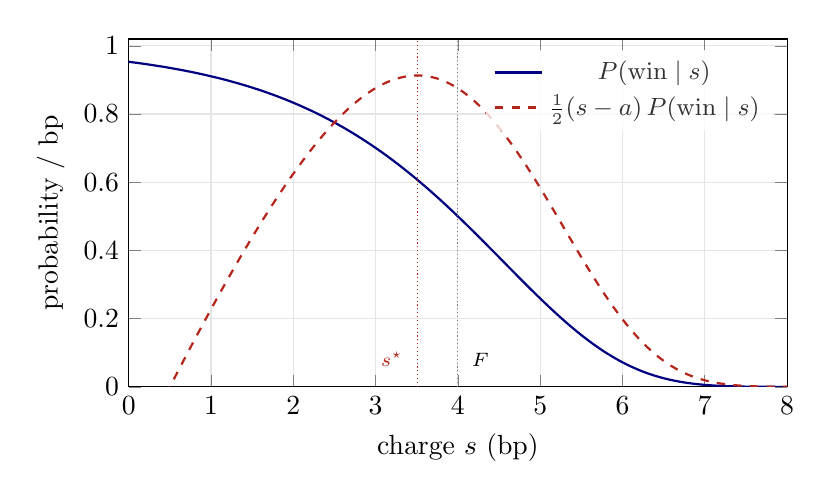
\begin{tikzpicture}
\begin{axis}[
  width=0.82\textwidth,height=6cm,
  xlabel={charge $s$ (bp)},
  ylabel={probability / bp},
  xmin=0,xmax=8,ymin=0,ymax=1.02,
  legend style={at={(0.98,0.97)},anchor=north east,font=\small,draw=none,fill=white,fill opacity=0.8},
  grid=major,grid style={gray!20},
  samples=200,domain=0:8]
\addplot[thick,NavyBlue] {exp(-exp((x-4)/1.5 + ln(ln(2))))};
\addlegendentry{$P(\text{win}\mid s)$}
\addplot[thick,BrickRed,dashed] {(x-0.5)*exp(-exp((x-4)/1.5 + ln(ln(2))))/2};
\addlegendentry{$\tfrac12(s-a)\,P(\text{win}\mid s)$}
\addplot[gray,densely dotted] coordinates {(4,0) (4,1.02)};
\addplot[BrickRed,densely dotted] coordinates {(3.507,0) (3.507,1.02)};
\node[font=\scriptsize,anchor=south west] at (axis cs:4.05,0.03) {$F$};
\node[font=\scriptsize,anchor=south east,BrickRed] at (axis cs:3.45,0.03) {$s^\star$};
\end{axis}
\end{tikzpicture}
\caption{Win curve and (scaled) expected margin for the worked example. The optimal quote sits inside the fair charge because filled tickets cost only $a=0.5$\,bp.}
\end{figure}

%======================================================================
\section{Validation and monitoring}\label{sec:validation}
%======================================================================

\begin{enumerate}[itemsep=2pt]
\item \textbf{Proper scoring.} Out-of-sample log score of the full likelihood, against two benchmarks: a pooled model without client effects, and a logistic win/loss classifier on the same features.
\item \textbf{Calibration of the win curve.} Reliability diagram of predicted $\pi_iS_C(s_i)$ against realised wins, by decile and by tier, venue, country and session.
\item \textbf{Shape of the cover.} Within cells, estimate $\hat S$ nonparametrically (Turnbull estimator on the interval table) and plot $\ln(-\ln\hat S(y))$ against $y$, or against $k=(y-F_i)/\sigma_i$ after standardisation. Under the model the plot is a straight line of slope $1/\sigma$ (Proposition~\ref{prop:ph}); curvature indicates a wrong family, a kink at small $n_i$ indicates the small-dealer-count issue of \S\ref{sec:limitations}. For exact and interval records, the randomised PIT $u_i=S_C(c_i)$ should be uniform.
\item \textbf{Family comparison.} Log score of Gumbel-min against the logistic (Proposition~\ref{prop:logistic}) on the same structure.
\item \textbf{Intraday filter.} One-step-ahead predictive log score of the filtered model versus the static morning model on replayed days; the filter must win on volatile days and not lose on quiet ones.
\item \textbf{Stability.} Day-over-day changes of multipliers, country curves and idiosyncratic spreads relative to their posterior standard deviations; persistent large moves indicate missing features, a mis-tuned half-life or a curvature penalty that is too weak.
\item \textbf{Economic backtest.} Realised P\&L and mark-outs of the policy \eqref{eq:optimal} versus the traders' actual quotes on a holdout period, acknowledging that off-policy evaluation is only partially identified (Section~\ref{sec:practical}).
\end{enumerate}

%======================================================================
\section{Practical issues}\label{sec:practical}
%======================================================================

\begin{description}[itemsep=3pt,leftmargin=0pt]
\item[Reference mid quality.] Every charge is relative to $m_i$. Errors in the mid are common to $s_i$ and $C_i$, so they do not affect the win/loss comparison, but they add noise to the level of $C_i$. Feed mid-quality indicators into the scale \eqref{eq:scale} and into $\delta_i$, and consider fitting separately by mid source.
\item[Endogeneity of our quotes.] Assumption~\ref{ass:censoring} fails if traders use information not in $\bx_i$. Mitigations: include what traders see (composite and evaluated prices, axes, recent prints, recent hit ratio); rely on exact observations ($\Wc$, $\Dl$), which are not affected by the censoring mechanism; and, once the model is live, add small random dither to quotes, which provides exogenous variation in $s_i$ and protects identification of the scale.
\item[Tape matching.] Post-trade transparency regimes cap disclosed sizes and allow deferred publication, which delays and blurs matches for large tickets. Encode this in $\rho_i$ and $\delta_i$ rather than discarding the observations; size-capped prints are still informative about the level.
\item[New and rarely quoted bonds.] They start on their country curve ($e_b=0$, full prior variance). A new issue that is systematically tighter or wider than its curve is learned through $e_b$ within the day by the intraday filter and across days by the morning fit.
\item[Sparse countries.] With few bonds the curve reduces to a line whose slope is pooled across countries; with one bond, the country level is pooled toward $\beta_0$.
\item[Inquiries we did not quote.] They are $\Dl$ or $\Dn$ observations with $s_i=+\infty$, informative about $C$ when a level is matched; include them, with a flag, if the reason for not quoting is unrelated to price.
\end{description}

%======================================================================
\section{Implementation checklist}
%======================================================================
\begin{enumerate}[itemsep=2pt]
\item Data layer: inquiry table with the fields of Section~1; charge mapping \eqref{eq:charge}; tape matcher producing $(c_i,\delta_i,\rho_i)$; interval table (Table~\ref{tab:intervals}).
\item Curve layer: daily nodes per country, $\bm D_g$, $\bm H_g$, $\bm K_g$ (Appendix~\ref{app:curve}); level/slope/shape decomposition \eqref{eq:levelslope}.
\item Model layer: sparse design matrices \eqref{eq:design}; unified interval log-likelihood with $\lmexp$; objective \eqref{eq:objective} in autodiff; unit tests of gradients against Appendix~\ref{app:derivatives}.
\item Morning job: Algorithm~\ref{alg:daily}; sparse Laplace covariance; publish Table~\ref{tab:outputs}.
\item Intraday service: state construction, prediction \eqref{eq:dyn}, Newton step \eqref{eq:newton}, update \eqref{eq:update}; delayed-tape handling; safeguards; logging of every update.
\item Quote layer: $F_i$ from \eqref{eq:multiplicative}, predictive curve \eqref{eq:predictive}, optimal quote \eqref{eq:optimal} or target-hit quote \eqref{eq:target}.
\item Validation suite of Section~\ref{sec:validation}, run nightly.
\end{enumerate}

\appendix
%======================================================================
\section{Derivatives of the likelihood terms}\label{app:derivatives}
%======================================================================
Write $w=e^{z}$, $S(z)=e^{-w}$ and $\varphi(z)=we^{-w}=-dS/dz$, with $d\varphi/dz=\varphi(1-w)$. Let $\mathcal D$ denote the derivative with respect to a common shift of all $z$-arguments (all arguments of one inquiry move together when $F_i$ moves).

\begin{center}\small
\renewcommand{\arraystretch}{1.6}
\begin{tabular}{llll}
\toprule
Type & $\ell(z)$ & $\mathcal D\ell$ & $\mathcal D^2\ell$ \\
\midrule
Right-censored ($\Win$) & $-w$ & $-w$ & $-w$ \\
Exact (density) & $z-w-\ln\sigma$ & $1-w$ & $-w$ \\
Left-censored ($\Dn$) & $\ln(1-e^{-w})$ & $\dfrac{w}{e^{w}-1}$ & $\dfrac{w\,(e^{w}-1-we^{w})}{(e^{w}-1)^2}$ \\
Interval $[z_a,z_b]$ & $\ln(S_a-S_b)$ & $\dfrac{\varphi_b-\varphi_a}{S_a-S_b}$ & $\dfrac{\varphi_b(1-w_b)-\varphi_a(1-w_a)}{S_a-S_b}-(\mathcal D\ell)^2$ \\
\bottomrule
\end{tabular}
\end{center}

For a mixture $\ell=\ln\bigl(\sum_jc_jL_j\bigr)$ (tape fallback \eqref{eq:mixture}, or contamination $\tilde S$, where the constant term has $\mathcal D L_j=0$), $\mathcal D\ell=\sum_j\omega_j\mathcal D\ell_j$ and $\mathcal D^2\ell=\sum_j\omega_j\bigl(\mathcal D^2\ell_j+(\mathcal D\ell_j)^2\bigr)-(\mathcal D\ell)^2$, with posterior weights $\omega_j=c_jL_j/\sum_kc_kL_k$.

\textbf{Chain rule.} In the daily fit, $\partial z/\partial F_i=-1/\sigma_i$ and $\partial z/\partial\ln\sigma_i=-(z-\zm)$, then linear maps to $\btheta$. In the intraday filter, with $\sigma_i$ frozen, \eqref{eq:chain_r} applies.

%======================================================================
\section{Order statistics for the dealer model}\label{app:orderstat}
%======================================================================
Under Assumption~\ref{ass:iid}, with $S_Q$ the survival of one competitor and $N=n_i-1$:
\begin{align*}
S_C(y)&=S_Q(y)^{N}, &&\text{(cover)}\\
\Prob(\text{exactly one competitor below } s)&=N\,F_Q(s)\,S_Q(s)^{N-1}, &&\text{(we are second, $\Dcv$)}\\
f_{C^{(2)}}(y)&=N(N-1)\,F_Q(y)\,S_Q(y)^{N-2}f_Q(y), &&\text{(second-best competitor)}.
\end{align*}
For Gumbel-min $Q$ with median $F^Q$, the cover is Gumbel-min with median $F^Q-\sigma\ln N$, which is \eqref{eq:dealers}.

%======================================================================
\section{Curvature penalty matrix}\label{app:curve}
%======================================================================
For country $g$ with nodes $\tau_1<\dots<\tau_J$ and gaps $\Delta_j=\tau_j-\tau_{j-1}$, row $j-1$ ($j=2,\dots,J-1$) of $\bm D_g\in\R^{(J-2)\times J}$ has three non-zeros:
\[
(\bm D_g)_{j-1,\,j-1}=\frac{2}{(\Delta_j+\Delta_{j+1})\Delta_j},\quad
(\bm D_g)_{j-1,\,j}=-\frac{2}{\Delta_j\Delta_{j+1}},\quad
(\bm D_g)_{j-1,\,j+1}=\frac{2}{(\Delta_j+\Delta_{j+1})\Delta_{j+1}},
\]
and $\bm H_g=\operatorname{diag}\bigl((\Delta_j+\Delta_{j+1})/2\bigr)_{j=2}^{J-1}$. Then $\bm K_g=\bm D_g\T\bm H_g\bm D_g$ is symmetric positive semi-definite and pentadiagonal, with null space spanned by $\bm1$ and $\bm\tau=(\tau_1,\dots,\tau_J)\T$. Each row of $\bm D_g$ sums to zero and annihilates $\bm\tau$, which is why level and slope are unpenalised and carried by $(a_g,b_g)$ in \eqref{eq:levelslope}. With equal gaps $\Delta$ the rows reduce to $(1,-2,1)/\Delta^2$, the familiar second difference.

The constraint $\tilde{\bff}_g\perp\{\bm1,\bm\tau\}$ is imposed by writing $\tilde{\bff}_g=\bm Z_g\bm\gamma_g$ with $\bm Z_g\in\R^{J\times(J-2)}$ an orthonormal basis of the orthogonal complement of $\{\bm1,\bm\tau\}$, computed once per day by QR; the penalty becomes $\tfrac{\lambda_g}{2}\bm\gamma_g\T(\bm Z_g\T\bm K_g\bm Z_g)\bm\gamma_g$, which is positive definite.

\end{document}
